\documentclass[conference]{IEEEtran}

\usepackage{amsmath}
\usepackage{amssymb}
\usepackage{booktabs}
\usepackage{array}
\usepackage{graphicx}
\usepackage{multirow}
\usepackage{url}
\usepackage{cite}
\usepackage{xcolor}
\usepackage{xspace}
\usepackage[hidelinks]{hyperref}
\usepackage{tikz}
\usetikzlibrary{positioning,arrows.meta,fit,calc,backgrounds}
\usepackage{tabularx}
\usepackage{threeparttable}

\newcommand{\code}[1]{\texttt{#1}}

\def\BibTeX{{\rm B\kern-.05em{\sc i\kern-.025em b}\kern-.08em
    T\kern-.1667em\lower.7ex\hbox{E}\kern-.125emX}}

% Global Float Padding Reduction
\setlength{\textfloatsep}{6pt plus 1.0pt minus 2.0pt}
\setlength{\floatsep}{6pt plus 1.0pt minus 2.0pt}
\setlength{\intextsep}{6pt plus 1.0pt minus 2.0pt}


\begin{document}

\title{Pre-Authorization Risk Screening for Blockchain Account Delegation under EIP-7702 with Hierarchical Bytecode Learning}



\maketitle

\begin{abstract}
Ethereum's EIP-7702 allows externally owned accounts to delegate code execution to smart-contract logic, creating a security decision point before the user authorizes the delegate. At authorization time, behavioral history, reputation information, or verified source code may be unavailable, while the delegate's deployed runtime bytecode is already observable. Existing EIP-7702 studies primarily examine attacks through transaction analysis, static analysis, or protocol-level defenses, while prior machine-learning work addresses general vulnerability or phishing-contract classification. To the best of our knowledge, AuthGuard-7702 is the first machine-learning framework designed specifically to screen EIP-7702 delegate runtime bytecode before authorization. Its core model, AuthGuard-Seq, is a lightweight 181,877-parameter hierarchical architecture that uses local convolutional encoders and learned chunk attention to capture ordered opcode patterns and aggregate evidence across long runtime programs. We evaluate AuthGuard-Seq on an audited corpus of 2,190 observed delegates partitioned into 790 bytecode-similarity families. Across five family-disjoint cross-validation folds and three training seeds, it achieves $0.924\pm0.014$ area under the precision--recall curve (AUPRC) and $0.833\pm0.016$ recall at the nominal 5\% false-positive-rate (FPR) operating point, ranking first among seven traditional and neural models. AuthGuard-Seq retains 0.920 AUPRC under a 200\% bytecode-flooding condition, while the complete measured local CPU screening path has a median latency of 4.121 ms. These results establish AuthGuard-7702 as a lightweight pre-authorization triage layer for secure blockchain account delegation at the EIP-7702 authorization boundary.
\end{abstract}

\begin{IEEEkeywords}
EIP-7702, Ethereum, smart contract security, bytecode analysis, machine learning
\end{IEEEkeywords}

\section{Introduction}
\label{sec:intro}

Ethereum traditionally distinguishes externally owned accounts (EOAs), which are controlled by users, from smart contracts that contain executable logic. EIP-7702 modifies this model by allowing an EOA to delegate code execution while retaining its original address~\cite{eip7702}. This enables account-abstraction capabilities such as transaction batching, gas sponsorship, and programmable authorization, but it also creates a new trust boundary. Authorizing unsafe delegate code can allow untrusted smart-contract logic to access or manipulate the EOA's state, assets, approvals, and transaction behavior.

The critical decision occurs before authorization. A newly proposed delegate may have little transaction history, no established reputation, and no verified source code, yet its deployed runtime bytecode can already be retrieved from the blockchain. Existing EIP-7702 studies document delegation-based phishing, persistent compromise, and related risks~\cite{qi2025eip7702,huang2026darkside}, but primarily emphasize ecosystem-scale detection, transaction evidence, static program analysis, or protocol defenses. In parallel, machine-learning studies show that EVM bytecode and opcode representations contain useful signals for vulnerability and phishing detection~\cite{phishinghook2025,contractward2021,eth2vec2022}. These approaches do not address the distinct operational decision of whether a proposed EIP-7702 delegate should be authorized. Figure~\ref{fig:riskwindow} illustrates this authorization risk window. The wallet can retrieve delegate runtime bytecode before signature, while behavioral, reputation-based, or source-level evidence may still be unavailable.

\begin{figure}[t]
\centering
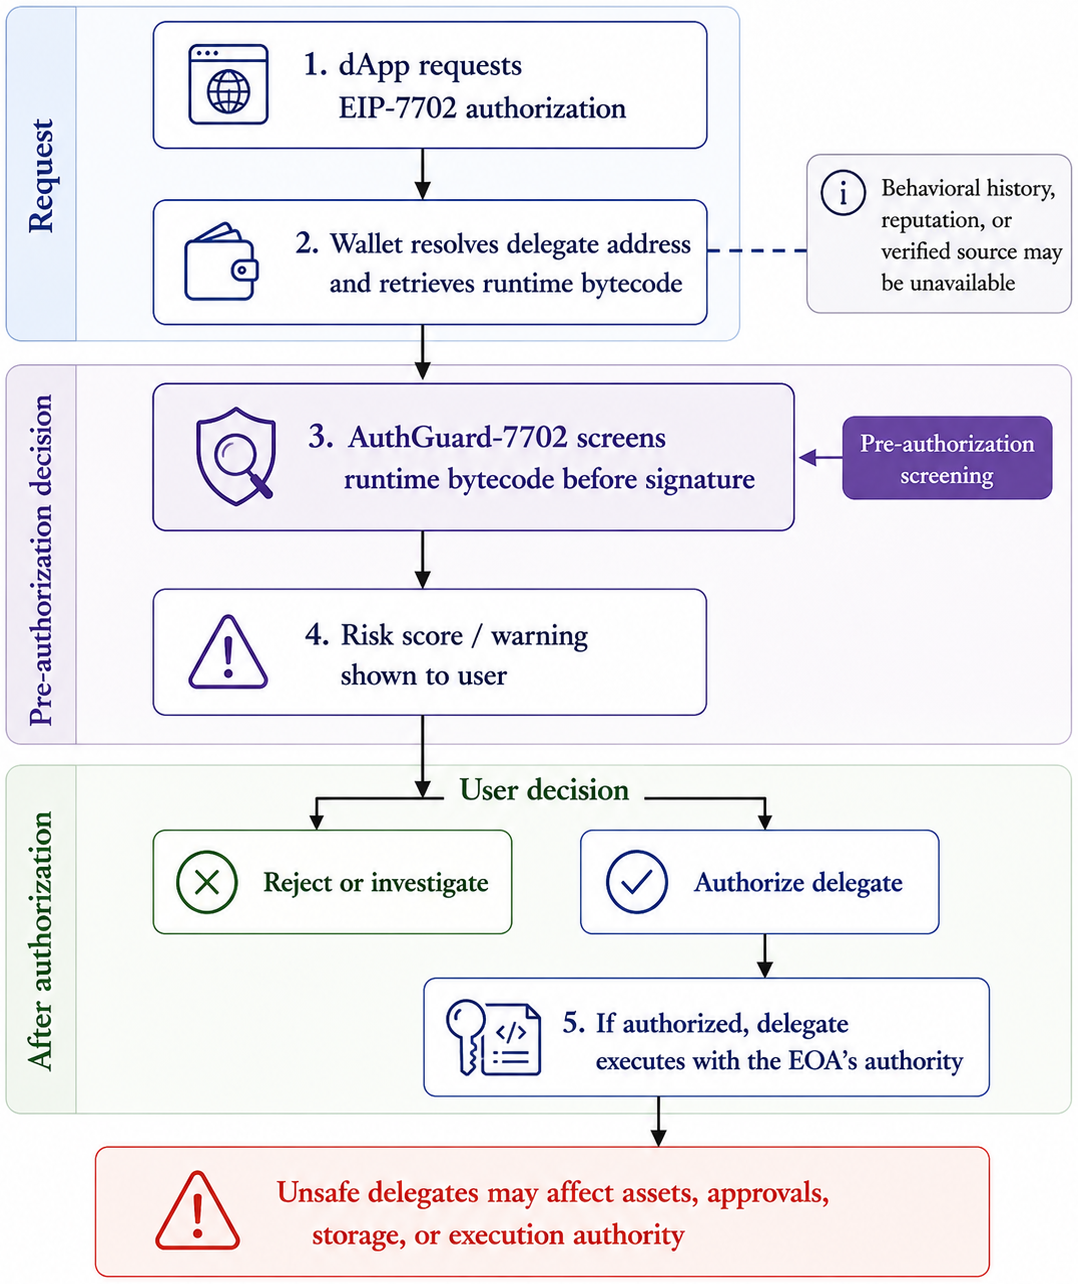
\includegraphics[width=\columnwidth]{eip_7702_authorization_risk_flowchart.png}
\caption{EIP-7702 authorization flow}
\label{fig:riskwindow}
\end{figure}

We address this gap with AuthGuard-7702, a bytecode-only pre-authorization screening framework that produces a calibrated screening score and warning tier. Its central model, AuthGuard-Seq, disassembles runtime bytecode, partitions the opcode stream into 256-token chunks, encodes local ordered patterns using shared convolutions, and learns attention weights that aggregate evidence across chunks. The model processes up to 16,384 opcodes, which is sufficient for every program in the audited benchmark, without using transaction history, source code, address identity, or reputation metadata.

A second methodological challenge is dependence among smart-contract samples. Code duplication can inflate the measured performance of machine-learning models of code~\cite{allamanis2019duplication}. Smart-contract datasets may likewise contain identical redeployments and closely related bytecode variants, allowing row-level random splits to place near-duplicate programs in both training and test data and thereby overstate generalization~\cite{tesseract2019}. We therefore audit the source data, construct bytecode-similarity families, prevent identical bytecode and related families from crossing folds, and exclude observations with unreliable source verdicts. On a primary benchmark of 2,190 observed delegates, AuthGuard-Seq achieves $0.924\pm0.014$ AUPRC and $0.833\pm0.016$ recall at the nominal 5\% FPR operating point. Family-clustered paired bootstrap confidence intervals support the observed improvements over Flat CNN and histogram+n-gram XGBoost. AuthGuard-Seq also retains AUPRC above 0.91 under the defined flooding and representation-stress conditions, while the complete measured local screening path has a median latency of 4.121 ms on one CPU thread.

The study makes three primary contributions:
\begin{itemize}
    \item To the best of our knowledge, we introduce the first machine-learning framework specifically designed to screen EIP-7702 delegate runtime bytecode before authorization, without requiring transaction history, reputation information, or verified source code.
    \item We develop AuthGuard-Seq, a compact 181,877-parameter hierarchical model that combines local opcode-order modeling with contract-wide chunk aggregation and outperforms six traditional and neural baselines under family-disjoint evaluation.
    \item We construct an audited benchmark and evaluation protocol combining duplicate and family controls, family-disjoint cross-validation, clustered statistical analysis, robustness testing, external controls, and local latency measurement.
\end{itemize}

\section{Background and Related Work}
\label{sec:related}
This section reviews the EIP-7702 authorization model and positions AuthGuard-7702 relative to prior bytecode learning, static analysis, and security-ML evaluation methodology.

\subsection{EIP-7702 and the Authorization Boundary}

EIP-7702 introduces authorization tuples through which an EOA can delegate code execution while retaining its original address. For each valid tuple, a delegation indicator formatted as $\code{0xef0100}\Vert\code{address}$ is written to the authorizing EOA's code field. Subsequent code-executing operations resolve and execute the code at the referenced delegate address~\cite{eip7702}. The security-relevant object for screening is therefore the delegate's executable runtime bytecode rather than the 23-byte indicator itself. Once authorized, the referenced code can execute in the EOA's context, making the pre-signature decision a natural point for automated screening.

Huang et al. combine transaction analysis with cross-contract static analysis to characterize EIP-7702-related malicious behavior~\cite{huang2026darkside}, while Qi et al. study delegation-based phishing mechanisms and protocol-level defenses~\cite{qi2025eip7702}. To the best of our knowledge, neither work investigates machine-learning-based screening of proposed delegate bytecode before authorization.

\subsection{Learning from Smart-Contract Bytecode}

Prior learning-based methods demonstrate that EVM representations can support security classification. ContractWard uses opcode bigrams with conventional learners~\cite{contractward2021}, Eth2Vec learns contract-wide bytecode representations~\cite{eth2vec2022}, and PhishingHook evaluates bytecode and opcode representations for phishing-contract classification~\cite{phishinghook2025}. More recent work combines bytecode-derived features with control-flow-graph analysis~\cite{smartbugbert2025}, while surveys emphasize representation, dataset construction, and evaluation design as recurring determinants of reported performance~\cite{wang2026review}. PhishingHook is particularly relevant because it shows that predictive security signals can be learned directly from EVM bytecode without transaction analysis. AuthGuard-7702 addresses a different operational setting by screening a proposed EIP-7702 delegate before authorization, and its primary benchmark consists entirely of observed delegates drawn from a common acquisition pipeline. Table~\ref{tab:related} summarizes this positioning.

\begin{table}[t]
\centering
\caption{Comparison with representative prior work}
\label{tab:related}
\begin{threeparttable}
\scriptsize
\begin{tabularx}{\columnwidth}{@{}X c c c@{}}
\toprule
Work & EIP-7702 & Bytecode ML & Pre-authorization screening \\
\midrule
Huang et al.~\cite{huang2026darkside} & \checkmark & -- & -- \\
Qi et al.~\cite{qi2025eip7702} & \checkmark & -- & -- \\
PhishingHook~\cite{phishinghook2025} & -- & \checkmark & -- \\
Eth2Vec~\cite{eth2vec2022} & -- & \checkmark & -- \\
\textbf{AuthGuard-7702} & \checkmark & \checkmark & \checkmark \\
\bottomrule
\end{tabularx}
\begin{tablenotes}[flushleft]
\scriptsize
\item[] ``Bytecode ML'' denotes machine learning directly over bytecode or opcode representations. ``Pre-authorization screening'' denotes automated risk assessment of proposed delegate code before authorization.
\end{tablenotes}
\end{threeparttable}
\end{table}

\subsection{Static Analysis and Security-ML Evaluation}

Bytecode learning complements rather than replaces semantic analysis. Gigahorse decompiles EVM bytecode for declarative analysis~\cite{gigahorse2019}, while Securify derives semantic dependencies and checks security patterns~\cite{securify2018}. The reference labels originate from a decompiler-based rule~\cite{huang2026darkside}, but our question is whether that signal can be approximated directly from opcode sequences by a lightweight pre-authorization screener. Evaluation methodology is equally important. TESSERACT shows how dependence and distribution bias can inflate security-classification results~\cite{tesseract2019}. We therefore isolate identical and similar bytecode families across folds and interpret transformed executable inputs only within their demonstrated preservation guarantees, consistent with problem-space adversarial-ML guidance~\cite{pierazzi2020}.



\begin{figure*}[t]
\centering
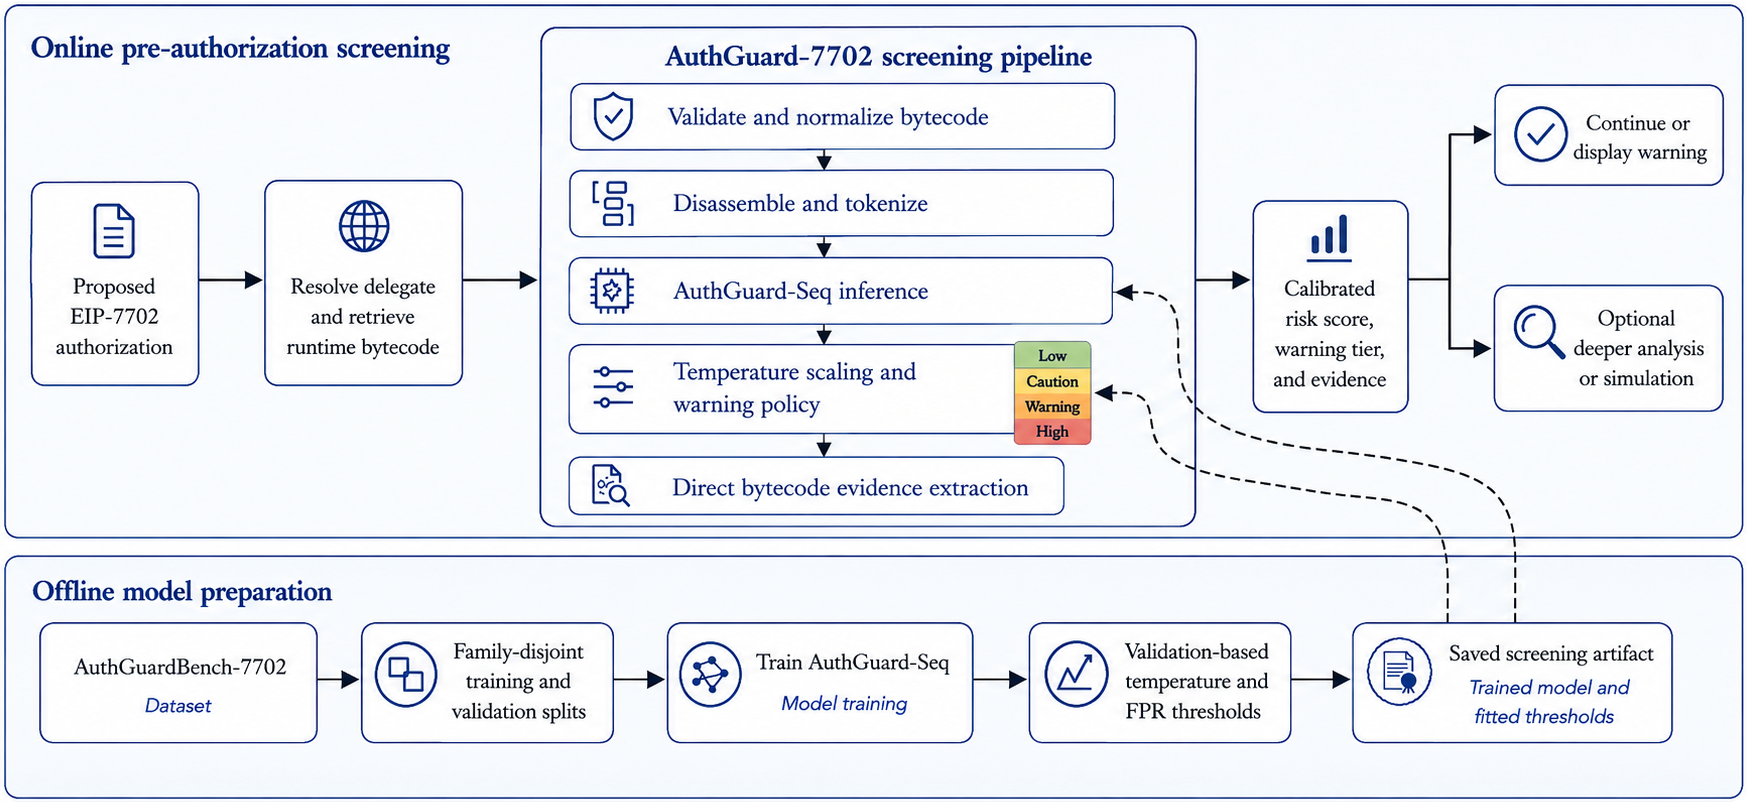
\includegraphics[width=0.98\textwidth]{figure-1-bak.png}
\caption{AuthGuard-7702 system overview}
\label{fig:decision}
\end{figure*}



\section{Problem Formulation and Threat Model}
\label{sec:problem}
This section defines the pre-authorization screening task, the model's information boundary, and the assumed attacker and defender capabilities.


\subsection{Pre-Authorization Screening Task}

Let $b$ denote the normalized runtime bytecode at a proposed delegate address and let $T(b)$ denote its opcode-token sequence. A trained model $f_\theta$ produces a risk logit that is temperature-scaled using validation data~\cite{guo2017calibration}:

\begin{equation}
s(b)=\sigma\left(\frac{f_\theta(T(b))}{T_{\mathrm{cal}}}\right),
\qquad
T_{\mathrm{cal}}>0,
\qquad
s(b)\in[0,1].
\label{eq:score}
\end{equation}

The resulting value $s(b)$ is a calibrated model score indicating the strength of evidence that the delegate contains opcode patterns associated with the benchmark's reference risk condition. The positive class consists of delegates flagged by the source study's static-analysis rule, which identifies decompiled reachability from standardized inbound hooks, including \code{receive()}, \code{fallback()}, and token-reception callbacks, to predefined value-moving external-call patterns~\cite{huang2026darkside}. The negative class consists of delegates from the same source pool that were not flagged. Because an unflagged verdict does not establish benign semantics, the task is screening for source-analyzer-identified risk rather than proving malicious intent, exploitability, or delegate safety.

From negative validation scores, we derive thresholds $\tau_1\geq\tau_5\geq\tau_{10}$ for nominal 1\%, 5\%, and 10\% FPR operating points. Scores $s\geq\tau_1$ map to \textsc{High}, $\tau_5\leq s<\tau_1$ to \textsc{Warning}, $\tau_{10}\leq s<\tau_5$ to \textsc{Caution}, and $s<\tau_{10}$ to \textsc{Low-Observed-Risk}. Because thresholds are estimated from finite validation sets, held-out FPR can differ from the nominal target.

\subsection{Information Boundary}

The core model observes only the ordered opcode sequence derived from runtime bytecode. PUSH immediate operands are skipped, so the sequence representation captures opcode identities and ordering rather than embedded constants. The model receives no transaction history, balances or approvals, graph or address identity, source code, family or fold identifiers, or fields used to construct the reference labels. This boundary is deliberate because the intended use case is a delegate that may lack historical or identity-based evidence at authorization time. The component is an advisory first-stage screener and does not resolve proxy state, simulate transactions, infer off-chain intent, or certify authorization safety. Those signals can be supplied by downstream security systems after initial triage.


\begin{figure*}[t]
\centering
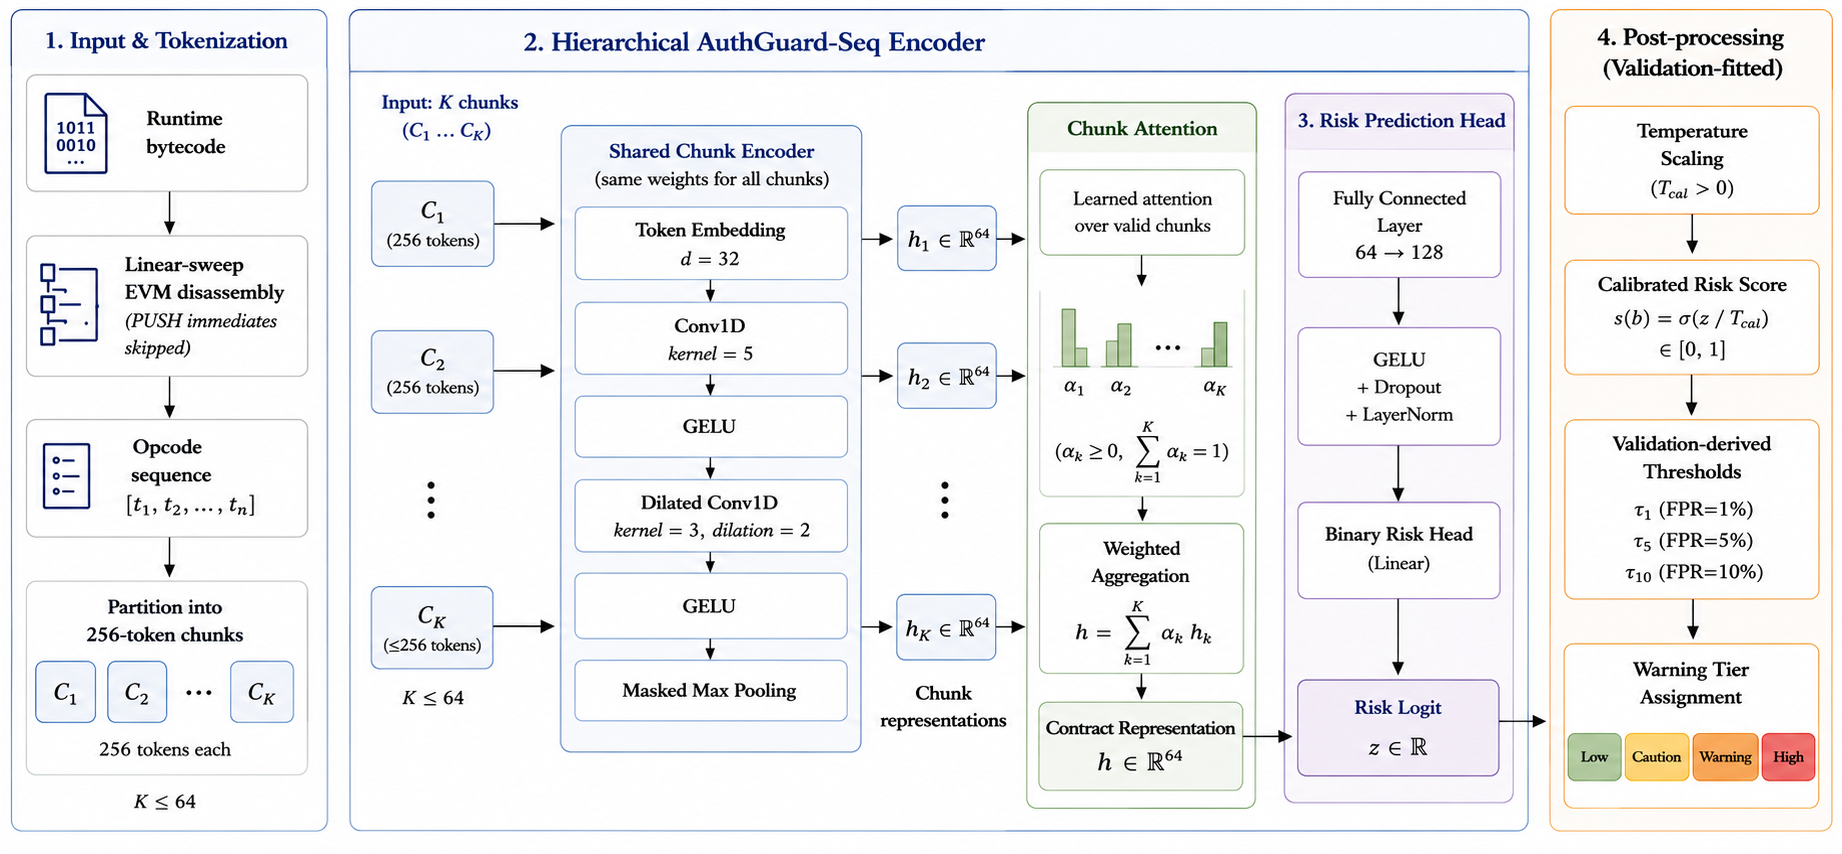
\includegraphics[width=0.98\textwidth]{figure-2-fixed.png}
\caption{AuthGuard-Seq architecture}
\label{fig:encoder}
\end{figure*}



\subsection{Threat Model}

We consider an adversary who attempts to induce authorization of a delegate whose runtime code exhibits the reference risk condition. The adversary may control the deployed bytecode and modify layout, appended content, metadata, or other representation-level features to evade bytecode screening. The defender is a wallet or security service that retrieves the proposed delegate's on-chain runtime bytecode and applies AuthGuard-7702 before authorization. We assume correct bytecode retrieval and trusted model parameters and screening code. Compromise of the wallet, signing key, retrieval infrastructure, or screener is outside the scope of this work.

The model can detect only risk signals observable from runtime bytecode. Behavior that depends primarily on dynamic state, transaction-specific context, unresolved proxy targets, external counterparties, or off-chain intent may remain invisible. Our robustness experiments therefore test selected representation-level modifications rather than universal robustness to arbitrary semantics-preserving or adaptive white-box transformations.



\section{AuthGuard-7702}
\label{sec:system}
This section presents the AuthGuard-7702 screening workflow and the hierarchical AuthGuard-Seq model used to assess delegate bytecode.



\subsection{Screening Workflow}

Figure~\ref{fig:decision} places AuthGuard-7702 at the EIP-7702 authorization boundary. A wallet or security service resolves the proposed delegate address, retrieves its runtime bytecode, and invokes the local screening path before the user authorizes it. The pipeline normalizes and disassembles the bytecode, runs AuthGuard-Seq, applies validation-fitted calibration and thresholds, and returns a risk score, warning tier, and auxiliary bytecode evidence. Elevated scores can trigger a wallet warning or deeper analysis before the authorization decision. During model development and evaluation, the offline path constructs family-disjoint folds, trains AuthGuard-Seq, and fits the temperature-scaling parameter and FPR thresholds using validation data only. The trained model, calibration parameter, and thresholds are then stored as the screening artifact used by the online path.



The auxiliary evidence is extracted separately from the raw bytecode and includes directly observed properties such as code length, opcode counts, call-family instructions, storage writes, contract-creation instructions, and recognized token-transfer or approval selectors. These observations and the learned attention weights provide context about influential bytecode regions, but they should not be interpreted as causal explanations or control-flow proofs.

\subsection{Design Requirements and Screening Semantics}

AuthGuard-7702 is designed as a bounded triage layer rather than a learned replacement for semantic analysis. The benchmark label encodes a decompiler-derived structural risk condition, while the deployed model receives only runtime opcode order. The learning problem is therefore deliberately constrained to determining whether a previously unseen delegate contains bytecode patterns associated with the reference condition without access to decompiler outputs, transaction history, source code, or identity information.

Table~\ref{tab:design-map} maps the principal deployment requirements to the mechanisms used by AuthGuard-Seq. Local convolutions preserve short opcode-order motifs, chunking supports long runtime programs, learned attention combines evidence distributed across chunks, and validation-fitted calibration and thresholds convert the raw model output into an operational warning policy.



At screening time, the saved model and calibration artifact are applied to the runtime bytecode resolved from the proposed delegate. A \textsc{Low-Observed-Risk} tier means only that the calibrated score lies below the lowest validation-derived threshold.  Higher tiers indicate progressively stronger model evidence and can be used by a wallet to display a warning or escalate the delegate to simulation, static analysis, or human review before authorization. Because the thresholds are fitted to validation FPR targets, their realized false-positive rates may shift when applied to a different contract population. RQ3 evaluates this transfer using an external benign-control population.



\begin{table}[t]
\centering
\caption{AuthGuard-Seq design requirements and corresponding mechanisms}
\label{tab:design-map}
\scriptsize
\begin{tabularx}{\columnwidth}{@{}X X X@{}}
\toprule
Requirement & Mechanism & Role \\
\midrule
Pre-authorization, bytecode-only use & Deterministic disassembly and opcode tokens & Operates without history or source code \\
Preserve local instruction order & Shared and dilated 1-D convolutions & Captures short ordered opcode motifs \\
Cover long runtime programs & Up to $64\times256$ opcode chunks & Processes up to 16,384 tokens without prefix-only truncation \\
Combine distributed evidence & Learned chunk attention & Produces a contract-level representation \\
Operational warning policy & Temperature scaling and validation-derived FPR thresholds & Maps calibrated scores to warning tiers \\
\bottomrule
\end{tabularx}
\end{table}



\subsection{Hierarchical Opcode-Sequence Model}

AuthGuard-Seq implements the preceding requirements using shared local convolutional encoders and contract-level chunk attention. The local encoders capture short ordered opcode patterns, while chunking and attention aggregate evidence across the processed runtime sequence. It begins with deterministic linear-sweep EVM disassembly. Recognized opcodes map to stable token IDs, undefined byte values use a dedicated token, and padding uses a separate ID. PUSH immediate operands are skipped according to their instruction widths. Tokenization does not terminate at the first linear \code{STOP} instruction, so trailing bytecode regions are not discarded solely because of an early stopping opcode. The resulting opcode sequence is divided into chunks of length $L=256$, with at most $K=64$ chunks. The longest benchmark program contains 16,081 opcodes and therefore fits within the model's 16,384-token capacity. Every benchmark contract is consequently processed in full. For longer contracts outside the benchmark, the model retains evenly spaced chunks rather than using prefix-only truncation.

Each chunk is embedded into 32 dimensions, processed by a kernel-5 convolution followed by a kernel-3 dilated convolution with dilation 2, and reduced through masked maximum pooling to a 64-dimensional representation $h_k$. Learned attention aggregates the valid chunk representations:

\begin{equation}
\alpha_k=\frac{\exp(w^\top h_k)}{\sum_{j=1}^{K_b}\exp(w^\top h_j)},
\qquad
h=\sum_{k=1}^{K_b}\alpha_k h_k,
\label{eq:attention}
\end{equation}


where $w$ is a learned vector and $K_b$ is the number of non-padding chunks. Larger values of $\alpha_k$ indicate greater learned relevance of chunk $k$ to the contract-level representation. The aggregated vector passes through a 128-dimensional fully connected layer with GELU activation, dropout, layer normalization, and a binary risk head. AuthGuard-Seq contains 181,877 trainable parameters. Its risk logit is temperature-scaled before the validation-derived warning thresholds are applied. Figure~\ref{fig:encoder} summarizes the architecture.




\section{Benchmark and Experimental Methodology}
\label{sec:method}
This section describes benchmark construction, family-disjoint evaluation, baselines, training, robustness testing, statistical analysis, and local timing measurement.

\subsection{Audited Benchmark Construction}
We have constructed {\it AuthGuardBench-7702}, an audited, family-disjoint EIP-7702 delegate-bytecode classification benchmark for evaluating pre-authorization risk screening models.
AuthGuardBench-7702 contains 3,082 audited observations partitioned into four populations before evaluation. The primary population comes from the EIP-7702 delegate dataset and analyzer outputs released by Huang et al.~\cite{huang2026darkside}. After auditing and filtering, it contains 2,190 delegates, including 727 source-analyzer-flagged and 1,463 source-unflagged observations. The external control contains 797 benign-labeled general Ethereum contracts from the PhishingHook-derived source~\cite{phishinghook2025}. Five manually curated legitimate EIP-7702 or account-abstraction implementations provide qualitative controls. Another 90 source observations are excluded because their original unflagged verdicts were produced from truncated or failed bytecode retrieval. Table~\ref{tab:dataset} summarizes these populations.

\begin{table}[t]
\centering
\caption{Audited benchmark populations and reference status}
\label{tab:dataset}
\scriptsize
\begin{tabularx}{\columnwidth}{@{}X r X r@{}}
\toprule
Population & $n$ & Reference status & Families \\
\midrule
Primary evaluation & 2,190 & 727 flagged / 1,463 unflagged & 790 \\
External benign control & 797 & Benign-labeled & -- \\
Qualitative control & 5 & Legitimate implementations & -- \\
Excluded uncertain input & 90 & Unreliable source verdict & -- \\
\midrule
Total audited rows & 3,082 & & \\
\bottomrule
\end{tabularx}
\end{table}

The primary flagged and unflagged classes come from the same EIP-7702 candidate pool and acquisition pipeline, which avoids confounding the main task with unrelated collection sources. They use the reference risk condition defined in Section~\ref{sec:problem}, and source-unflagged delegates are treated as weak negatives because rule silence does not establish benign semantics. During auditing, we identified 89 negative bytecodes truncated at the Excel cell limit and one timeout string stored instead of executable bytecode. Although the corresponding runtimes were recovered, all 90 observations were excluded because their original source verdicts had not been established on the repaired inputs. The benchmark therefore adds corrected filtering, duplicate handling, bytecode-family construction, external controls, and leakage-resistant splits to the source data.

\subsection{Families, Duplicates, and Splits}

Runtime bytecode is linearly disassembled and represented as opcode 4-gram sets. Deterministic 128-permutation BLAKE2b MinHash signatures with a fixed 0.85 signature-agreement threshold define similarity links, which are merged by union-find into 790 bytecode-similarity families. Identical bytecode with conflicting reference labels is quarantined before modeling.

We use five fixed family-disjoint outer folds. For test fold $f$, fold $(f+1)\bmod5$ serves as validation and the remaining three folds as training. No bytecode family or identical bytecode crosses outer folds. Each clean model is repeated with seeds 7702, 7703, and 7704. Results first average the five folds within each seed and then report the mean and sample standard deviation across the three seed-level means.

\subsection{Evaluation Validity Controls}

The evaluation protocol is structured to reduce several common sources of optimistic security-ML results. Table~\ref{tab:validity-controls} summarizes the controls and the specific bias each addresses. These controls are applied before reporting model comparisons, so the primary results measure transfer to held-out bytecode families rather than reuse of closely related deployments.

\begin{table}[t]
\centering
\caption{Evaluation-validity controls}
\label{tab:validity-controls}
\scriptsize
\begin{tabularx}{\columnwidth}{@{}X X@{}}
\toprule
Potential source of bias & Control \\
\midrule
Duplicate or near-duplicate leakage & Identical bytecode and similarity families remain within one outer fold, while conflicting duplicates are quarantined \\
Test-set tuning & Early stopping, temperature scaling, and FPR thresholds use validation data only \\
Correlated observations in uncertainty estimates & Paired bootstrap resamples bytecode families rather than individual rows \\
Cross-partition transformation leakage & Flooding donor pools are isolated by data partition and bytecode family \\
Unknown threshold transfer & Separate benign-labeled external controls and curated legitimate EIP-7702 examples are evaluated without fitting on them \\
\bottomrule
\end{tabularx}
\end{table}

\subsection{Baselines}

The clean comparison evaluates seven predefined model configurations under the same observations, family-disjoint folds, validation rotation, seeds, early-stopping policy, calibration, and operating-point construction. Table~\ref{tab:baseline-config} summarizes their representations and scales. Nonhierarchical neural sequence baselines use a 2,048-position opcode view obtained by uniform sampling, whereas AuthGuard-Seq processes the complete benchmark streams with at most 64 chunks of 256 tokens. Neural baselines use class-weighted binary cross-entropy and validation-AUPRC early stopping, so test performance does not influence training decisions. The comparison therefore evaluates the hierarchical full-stream design as a whole rather than isolating sequence coverage from aggregation. The robustness study retains AuthGuard-Seq, Flat CNN, and XGBoost as the proposed model, strongest clean neural baseline, and strongest traditional baseline.



\subsection{Training and Calibration}

Neural models use class-weighted binary cross-entropy, with positive-class weight equal to the training-fold negative-to-positive ratio. AuthGuard-Seq uses AdamW with learning rate $10^{-3}$, weight decay $10^{-4}$, batch size 16, gradient clipping at 5, and at most 30 epochs. Early stopping uses validation AUPRC with patience five. Temperature scaling~\cite{guo2017calibration} is then fit only on validation logits, and nominal 1\%, 5\%, and 10\% FPR thresholds are derived only from negative validation examples. Test labels are never used for model selection, calibration, or threshold construction.

\subsection{Robustness Protocol}

We compare clean bytecode with two transformed-input conditions. \textbf{Flood-200\%} appends a \code{STOP} instruction followed by deterministic donor bytes whose length equals 200\% of the source executable length. Donor pools are isolated by data partition and bytecode family to prevent cross-split leakage. In a bounded audit of 100 execution calls, no divergence was observed between the source and flooded inputs in the test harness's recorded execution behavior. We therefore treat Flood-200\% as having bounded empirical preservation support rather than universal semantic equivalence.

\textbf{Rewrite+Flood-200\%} additionally rewrites recognized metadata and selected embedded address and function-selector values before flooding. Because AuthGuard-Seq skips PUSH immediate bytes, these immediate-value rewrites do not directly alter its opcode-identity sequence. This combined condition is therefore a cross-model representation-stress test and is not assumed to preserve execution behavior universally. All transformed inputs are generated within their data partitions with family isolation preserved. Within each robustness run, clean and transformed inputs are evaluated using the same trained model and the same validation-derived operating points, so transformation effects are not confounded by retraining or threshold changes.


\begin{table}[t]
\centering
\caption{Baseline configurations}
\label{tab:baseline-config}
\scriptsize
\begin{tabularx}{\columnwidth}{@{}l X r@{}}
\toprule
Model & Input and model summary & Params. \\
\midrule
AuthGuard-Seq & Full opcode stream, 256-token chunks, $K\leq64$, local CNN and chunk attention & 181,877 \\
Flat CNN & 2,048 uniformly sampled opcodes, local 1-D convolutions and global pooling & 154,177 \\
XGBoost & 225-bin opcode histogram and 512-d hashed opcode 4-grams, 300 trees, depth 6 & -- \\
Neural n-gram & 512-d hashed opcode 4-gram view with neural classifier & 181,877 \\
BiGRU & 2,048 sampled opcodes, bidirectional recurrence and masked-mean readout & 108,225 \\
Dense structural & 261-d histogram and structural features with neural classifier & 181,877 \\
Transformer & 2,048 sampled opcodes, compact encoder with positional embeddings & 425,217 \\
\bottomrule
\end{tabularx}
\end{table}




\subsection{Metrics, Statistical Analysis, and Timing}

AUPRC is the primary ranking metric because the primary population is class-imbalanced and the metric emphasizes positive-class ranking. AUROC and calibrated Brier score are secondary metrics. Operational behavior is measured as Recall@5\% FPR, meaning recall at the threshold chosen from validation negatives for the nominal 5\% FPR target. For inferential comparisons, the bytecode family is the resampling unit. We perform 10,000 paired family-clustered percentile-bootstrap replicates with fixed seed 77022026. Families are resampled with replacement within each outer test fold, and the same resampling multiplicities are applied to both models in a pair. Metrics are computed per fold and seed, averaged across the five folds and then across the three training seeds, and reported with 95\% confidence intervals for paired differences.

For local timing, 300 contracts stratified across fold, label, and code-size order are each evaluated five times, producing 1,500 complete screening calls. Measurements use one thread on an AMD Ryzen 5 3600 with Python 3.12.12 and PyTorch 2.9.0. Model-load latency is summarized over 10 loads, and forward-only latency over 195 inference calls. The complete timed path includes validation, normalization, disassembly and tokenization, chunk construction, inference, calibration, warning assignment, evidence extraction, and response construction. RPC access, node latency, wallet rendering, user interaction, and external services are excluded.







\section{Evaluation}
\label{sec:evaluation}

We evaluate four questions: (RQ1) how accurately AuthGuard-Seq screens held-out EIP-7702 delegate families relative to traditional and neural baselines, (RQ2) how performance changes under bytecode flooding and representation stress, (RQ3) how validation-derived thresholds transfer to an external benign-control population, and (RQ4) whether local screening is lightweight enough for interactive use.

\subsection{RQ1: Clean Screening Effectiveness}

Table~\ref{tab:clean} reports the primary clean results as the mean $\pm$ standard deviation across the three seed-level fold means. AuthGuard-Seq ranks first with $0.924\pm0.014$ AUPRC, $0.963\pm0.011$ AUROC, and $0.072\pm0.012$ Brier score. At the nominal 5\% validation-negative FPR threshold, it achieves $0.833\pm0.016$ recall with held-out test FPR $0.052\pm0.007$. Flat CNN reaches $0.885\pm0.010$ AUPRC and $0.712\pm0.024$ Recall@5\% FPR, while histogram+n-gram XGBoost reaches $0.833\pm0.004$ and $0.615\pm0.015$, respectively. The ordering AuthGuard-Seq $>$ Flat CNN $>$ XGBoost $>$ neural n-gram is stable across all three seeds. BiGRU is substantially less stable, while the compact Transformer performs poorly at this dataset scale.

\begin{table}[t]
\centering
\caption{Clean family-disjoint performance}
\label{tab:clean}
\scriptsize
\begin{tabularx}{\columnwidth}{@{}X r r r r@{}}
\toprule
Model & AUPRC $\uparrow$ & AUROC $\uparrow$ & Brier $\downarrow$ & Recall@5\% FPR $\uparrow$ \\
\midrule
\textbf{AuthGuard-Seq} & \textbf{.924$\pm$.014} & \textbf{.963$\pm$.011} & \textbf{.072$\pm$.012} & \textbf{.833$\pm$.016} \\
Flat CNN & .885$\pm$.010 & .937$\pm$.007 & .099$\pm$.004 & .712$\pm$.024 \\
Hist.+4-gram XGBoost & .833$\pm$.004 & .907$\pm$.002 & .127$\pm$.003 & .615$\pm$.015 \\
Neural n-gram & .810$\pm$.007 & .880$\pm$.020 & .125$\pm$.001 & .654$\pm$.029 \\
BiGRU & .679$\pm$.098 & .815$\pm$.069 & .163$\pm$.027 & .379$\pm$.113 \\
Dense structural & .637$\pm$.018 & .780$\pm$.022 & .182$\pm$.009 & .331$\pm$.023 \\
Transformer & .563$\pm$.031 & .730$\pm$.019 & .208$\pm$.013 & .239$\pm$.054 \\
\bottomrule
\end{tabularx}
\end{table}

Paired family-clustered analysis supports the ranking. Against Flat CNN, AuthGuard-Seq improves AUPRC by $+0.039$ with 95\% CI $[+0.009,+0.073]$ and Recall@5\% FPR by $+0.121$ with CI $[+0.050,+0.190]$. Against XGBoost, the corresponding gains are $+0.091$ AUPRC with CI $[+0.045,+0.140]$ and $+0.217$ recall with CI $[+0.124,+0.314]$.

\subsection{RQ2: Robustness to Bytecode Transformation}

Table~\ref{tab:robust} summarizes transformed-input performance. Under Flood-200\%, AuthGuard-Seq retains $0.920\pm0.007$ AUPRC and $0.747\pm0.024$ Recall@5\% FPR. Under Rewrite+Flood-200\%, it reaches $0.912\pm0.005$ and $0.745\pm0.023$. Flat CNN and XGBoost degrade sharply under both conditions.



Under Flood-200\%, AuthGuard-Seq exceeds Flat CNN by $+0.385$ AUPRC with CI $[+0.302,+0.472]$ and XGBoost by $+0.344$ with CI $[+0.286,+0.397]$. The corresponding Recall@5\% FPR gains are $+0.556$ with CI $[+0.463,+0.655]$ and $+0.521$ with CI $[+0.442,+0.607]$. Under Rewrite+Flood-200\%, AUPRC advantages are $+0.387$ over Flat CNN and $+0.355$ over XGBoost, with both confidence intervals excluding zero. Relative to matched clean models from the same robustness run, AuthGuard-Seq AUPRC decreases by 0.013 with CI $[-0.030,-0.002]$ under Flood-200\% and by 0.020 with CI $[-0.037,-0.009]$ under Rewrite+Flood-200\%. Recall decreases by approximately 0.104--0.105, indicating that ranking quality is more stable than low-FPR operating-point recall. These claims are limited to the defined transformation protocols.

\subsection{RQ3: External Benign-Control Behavior}

Applying the primary validation thresholds to 797 benign-labeled general Ethereum contracts yields FPRs of $0.015\pm0.004$, $0.065\pm0.012$, and $0.169\pm0.021$ at the nominal 1\%, 5\%, and 10\% operating points. The nominal 5\% threshold therefore transfers with an observed external-control FPR of $0.065\pm0.012$, indicating moderate transfer with measurable distribution shift. This population is an external benign control, not an independent EIP-7702 deployment distribution. The five curated legitimate EIP-7702 controls are too few for statistical estimation, but across the 15 cross-validation models their mean scores range from 0.077 to 0.270 and their fraction flagged at the 5\% threshold ranges from 0 to 0.067. We treat these controls as a qualitative sanity check only.

\subsection{RQ4: Operational Viability}

Table~\ref{tab:latency} reports the local CPU measurements. Across 1,500 complete screening calls, median latency is 4.121 ms, the 95th percentile is 14.547 ms, and the 99th percentile is 21.429 ms. Forward inference alone has 0.950 ms median latency, while model loading takes 7.690 ms median and can be amortized in a persistent process.




\begin{table}[t]
\centering
\caption{Transformed-input performance}
\label{tab:robust}
\scriptsize
\begin{tabularx}{\columnwidth}{@{}l X r r@{}}
\toprule
Condition & Model & AUPRC & Recall@5\% FPR \\
\midrule
\multirow{3}{*}{Flood-200\%}
& \textbf{AuthGuard-Seq} & \textbf{.920$\pm$.007} & \textbf{.747$\pm$.024} \\
& Flat CNN & .535$\pm$.013 & .191$\pm$.010 \\
& XGBoost & .576$\pm$.003 & .226$\pm$.014 \\
\midrule
\multirow{3}{*}{Rewrite+Flood-200\%}
& \textbf{AuthGuard-Seq} & \textbf{.912$\pm$.005} & \textbf{.745$\pm$.023} \\
& Flat CNN & .525$\pm$.011 & .185$\pm$.013 \\
& XGBoost & .557$\pm$.007 & .202$\pm$.014 \\
\bottomrule
\end{tabularx}
\end{table}



\begin{table}[t]
\centering
\caption{Local CPU latency}
\label{tab:latency}
\scriptsize
\begin{tabularx}{\columnwidth}{@{}X r r r r@{}}
\toprule
Scope & Calls & Median & p95 & p99 \\
\midrule
Full local screening & 1,500 & 4.121 ms & 14.547 ms & 21.429 ms \\
Model load & 10 & 7.690 ms & 9.716 ms & 10.574 ms \\
Forward only & 195 & 0.950 ms & 1.585 ms & -- \\
\bottomrule
\end{tabularx}
\end{table}

The timed checkpoint contains 181,877 parameters and occupies 742,625 bytes. It is the seed-7702, fold-0 cross-validation artifact used for timing rather than a final retrained deployment model. These measurements cover local screening only and exclude network access, node response time, wallet rendering, and user interaction.

\section{Discussion and Limitations}
\label{sec:discussion}
This section interprets the findings in the context of an EIP-7702 defense stack and discusses the principal limitations of the study.

\subsection{Implications for an EIP-7702 Defense Stack}

The results support a division of labor between rapid learned screening and deeper semantic analysis. When a proposed delegate's runtime bytecode is available but behavioral context remains sparse, a wallet can use AuthGuard-7702 to prioritize higher-risk delegates for static analysis, symbolic execution, transaction-history checks, or human review rather than treat the learned model as a deterministic proof engine.

The baseline ordering is consistent with opcode order providing useful predictive information. Flat CNN outperforms histogram, hashed n-gram, and dense structural baselines, while AuthGuard-Seq remains markedly stronger under bytecode flooding. Local convolutions may capture short ordered patterns, while the hierarchical design aggregates evidence across a longer runtime view. Because the experiments evaluate the full architecture, isolating the effects of attention, chunking, and sequence coverage remains future work.

AuthGuard-7702 complements rather than replaces formal or semantic analysis. It approximates the benchmark's reference risk signal from opcode sequences, whereas Gigahorse recovers richer program semantics~\cite{gigahorse2019}. The learned stage provides rapid prioritization at the authorization boundary. We do not claim a runtime advantage over the source-analysis pipeline because this study evaluates only the effectiveness and operational feasibility of bytecode-based pre-authorization screening.

\subsection{Limitations and Future Work}

The reference labels encode a decompiler-based structural risk condition rather than independently adjudicated malicious intent, so AuthGuard-7702 is a triage model for that signal. Family-disjoint evaluation measures generalization to unseen bytecode lineages, but temporal generalization remains untested. The higher-than-nominal FPR on the external benign control at the 10\% operating point shows that calibration and threshold transfer can shift across populations. Robustness conclusions are limited to Flood-200\% and Rewrite+Flood-200\%, and the latter is a representation-stress condition rather than a universally semantics-preserving transformation. Local timing does not represent end-to-end wallet latency. Future work should evaluate adaptive transformations, representative external EIP-7702 controls, component ablations, and wallet pipelines combining learned screening with dynamic and semantic analysis.

\section{Conclusion}
\label{sec:conclusion}

We presented AuthGuard-7702, a machine-learning framework for pre-authorization risk screening of EIP-7702 delegate bytecode, and AuthGuard-Seq, a compact hierarchical opcode-sequence model for long runtime programs. On an audited, family-disjoint benchmark of 2,190 observed delegates, AuthGuard-Seq achieved $0.924\pm0.014$ AUPRC and $0.833\pm0.016$ Recall@5\% FPR, ranking first among seven evaluated traditional and neural models. Paired family-clustered bootstrap confidence intervals support the observed improvements over Flat CNN and histogram+n-gram XGBoost. AuthGuard-Seq also remained the strongest evaluated model under both transformation conditions, while the complete local screening path had a median latency of 4.121 ms. These findings support AuthGuard-7702 as a practical bytecode-based triage layer that can complement deeper semantic and behavioral analysis before EIP-7702 authorization.

\begin{thebibliography}{00}

\bibitem{eip7702}
V. Buterin, S. Wilson, A. Dietrichs, and lightclient, ``EIP-7702: Set Code for EOAs,'' \emph{Ethereum Improvement Proposals}, no. 7702, May 2024. [Online]. Available: \url{https://eips.ethereum.org/EIPS/eip-7702}

\bibitem{huang2026darkside}
M. Huang, H. Liu, S. Yang, D. Wu, and S. Wang, ``Revealing the Dark Side of Smart Accounts: An Empirical Study of EIP-7702 Incurred Risks in Blockchain Ecosystem,'' in \emph{Proc. 35th USENIX Security Symposium (USENIX Security 26)}, 2026, to appear.

\bibitem{qi2025eip7702}
M. Qi, Q. Wang, R. Li, T. Zhu, and S. Chen, ``EIP-7702 Phishing Attack,'' \emph{arXiv preprint arXiv:2512.12174}, Dec. 2025.

\bibitem{phishinghook2025}
P. De Rosa, S. Queyrut, Y.-D. Bromberg, P. Felber, and V. Schiavoni, ``PhishingHook: Catching Phishing Ethereum Smart Contracts Leveraging EVM Opcodes,'' in \emph{Proc. 2025 55th Annu. IEEE/IFIP Int. Conf. Dependable Systems and Networks (DSN)}, Naples, Italy, 2025, pp. 222--232.

\bibitem{contractward2021}
W. Wang, J. Song, G. Xu, Y. Li, H. Wang, and C. Su, ``ContractWard: Automated Vulnerability Detection Models for Ethereum Smart Contracts,'' \emph{IEEE Trans. Netw. Sci. Eng.}, vol. 8, no. 2, pp. 1133--1144, Apr.--Jun. 2021.

\bibitem{eth2vec2022}
N. Ashizawa, N. Yanai, J. P. Cruz, and S. Okamura, ``Eth2Vec: Learning Contract-Wide Code Representations for Vulnerability Detection on Ethereum Smart Contracts,'' \emph{Blockchain: Research and Applications}, vol. 3, no. 4, art. no. 100101, Dec. 2022.

\bibitem{allamanis2019duplication}
M. Allamanis, ``The Adverse Effects of Code Duplication in Machine Learning Models of Code,'' in \emph{Proc. ACM Onward!}, 2019, pp. 143--153, doi: 10.1145/3359591.3359735.

\bibitem{tesseract2019}
F. Pendlebury, F. Pierazzi, R. Jordaney, J. Kinder, and L. Cavallaro, ``TESSERACT: Eliminating Experimental Bias in Malware Classification across Space and Time,'' in \emph{Proc. 28th USENIX Security Symposium (USENIX Security 19)}, Santa Clara, CA, USA, 2019, pp. 729--746.

\bibitem{smartbugbert2025}
J. Bu, W. Li, Z. Li, Z. Zhang, and X. Li, ``SmartBugBert: BERT-Enhanced Vulnerability Detection for Smart Contract Bytecode,'' \emph{arXiv preprint arXiv:2504.05002}, Apr. 2025.

\bibitem{wang2026review}
B. Wang, Y. Tong, S. Ji, H. Dong, X. Luo, and P. Zhang, ``A Review of Learning-Based Smart Contract Vulnerability Detection: A Perspective on Code Representation,'' \emph{ACM Trans. Softw. Eng. Methodol.}, vol. 35, no. 6, 2026, doi: 10.1145/3750042.

\bibitem{gigahorse2019}
N. Grech, L. Brent, B. Scholz, and Y. Smaragdakis, ``Gigahorse: Thorough, Declarative Decompilation of Smart Contracts,'' in \emph{Proc. 2019 IEEE/ACM 41st Int. Conf. Software Engineering (ICSE)}, Montreal, QC, Canada, 2019, pp. 1176--1186.

\bibitem{securify2018}
P. Tsankov, A. Dan, D. Drachsler-Cohen, A. Gervais, F. Bünzli, and M. Vechev, ``Securify: Practical Security Analysis of Smart Contracts,'' in \emph{Proc. 2018 ACM SIGSAC Conf. Computer and Communications Security (CCS)}, Toronto, ON, Canada, 2018, pp. 67--82.

\bibitem{pierazzi2020}
F. Pierazzi, F. Pendlebury, J. Cortellazzi, and L. Cavallaro, ``Intriguing Properties of Adversarial ML Attacks in the Problem Space,'' in \emph{Proc. 2020 IEEE Symp. Security and Privacy (SP)}, San Francisco, CA, USA, 2020, pp. 1332--1349.

\bibitem{guo2017calibration}
C. Guo, G. Pleiss, Y. Sun, and K. Q. Weinberger, ``On Calibration of Modern Neural Networks,'' in \emph{Proc. ICML}, 2017, pp. 1321--1330.

\end{thebibliography}

\end{document}